%!TEX root = paper.tex
\section{NebulaStream Platform Overview}
\label{nes}
In this demonstration, we focus on specific aspects of NES and provide a brief overview.
For a detailed description of NES, we refer the reader to our previous work~\cite{nes}.  
First, we outline the limitation of state-of-the-art cloud-based SPEs that prevent them from exploiting upcoming IoT infrastructures \Cref{adapting}.
After that, we describe NES and its architecture in \Cref{nes_arch}.
% 
\subsection{Limitation of State-of-the-art SPEs}
\label{adapting}
In the following, we discuss two important features that limit cloud-based SPEs to support future IoT scenarios.

\textbf{Exploitation of Intermediate Nodes:}
Intermediate nodes route sensor-generated data to the cloud.
In an IoT infrastructure, devices are heterogeneous. They range from low-budget processing devices, such as mobile phones and Raspberry PIs, to standard desktop computers and high-end processing nodes with GPUs. 
Current SPEs are unable to exploit all intermediate nodes, because applications must wait until generated data reaches the cloud. 
For example, consider a simple aggregation task, such as counting the number of potential passengers per geographical area. To execute this task, cloud-based systems would have to wait until intermediate nodes propagate the data to the cloud. However, in the described IoT infrastructure, intermediate nodes can execute this task before the data reaches the cloud.

\textbf{On-demand Data Acquisition:}
If the set of running queries does not require all incoming sensor data streams, it would be possible to avoid these sensor reads by employing acquisitional data processing~\cite{tinydb}. 
Additionally, by adapting the sampling frequency of each sensor based on the query requirements, we can reduce network traffic between sensors, and the cloud further.
For example, a vehicle could potentially acquire, and send its data only if it is located in a certain area.


%\subsection{Design Principles}
%\label{nes_chars}
%\textcolor{red}{(@TODO,remove this)}
%NES overcomes the previously introduced limitations of cloud-based SPEs by adhering to the following design principles: 
%\begin{itemize}
%  \item{NES reuses intermediate results both between and within queries, by operator and query-leve optimizations.}
%  \item{NES handles new queries and topology updates incrementally, instead of restarting deployment.}
%  \item{NES generates hardware-tailored code for heterogeneous processing nodes.}
%  \item{NES handles resource availability transparently by providing configurable SLAs.}
%  \item{NES exposes user-friendly interfaces, letting the user focus on business logic rather than system internals.}
%  \item{Every NES node receives the necessary means to react autonomously in case of failures.}
%\end{itemize}

\subsection{Architecture} 
\label{nes_arch}
In the following, we describe NES's architecture. 
We illustrate the architecture in \Cref{nes_architecture}, and focus only on the components that are related to our application scenario. 
Note that NES provides additional components, however, we omit their descriptions because they are out of the scope of this demonstration. 
We refer the reader to our recent work~\cite{nes} for more details.

\textbf{Optimization Process:} 
External Services, e.g., the visualization application from our scenario, submit queries to NES. NES provides APIs to describe common data processing operations, similarly to state-of-the-art SPEs but with fog-specific extensions. 
The \textit{Query Manager} manages and coordinates incoming queries. 
Query execution in NES proceeds as follows. 
First, NES translates the user queries to logical query plans. 
After that, the plan is handed over to NES's Optimizer. 
The \textit{NES Optimizer} consults the \textit{NES Topology Manager}, which monitors the infrastructure changes, and performance statistics. 
The NES Optimizer then composes the execution plan, which it then deploys to its nodes through the \textit{NES Deployment Manager}.
In case of new queries, or topology updates, the NES Deployment Manager applies required changes in an incremental fashion.

\textbf{Deployment and Execution:}
NES's execution plan maps segmented sub-plans to participating, processing intermediate, or cloud nodes. 
Each segment contains processing instructions (tasks), as well as input, and output information. The NES Deployment Manager is responsible for transmitting the sub-plans to each node. After receiving a sub-plan, a node sets up the necessary connections with other nodes, and starts the execution. 
Each node has its own task scheduler, which uses a thread pool, and assigns tasks alongside I/O operations to its resources. 

\textbf{Monitoring:}
During runtime, the NES Topology Manager monitors the execution, and reacts to changes incrementally, e.g., by transitioning smoothly between execution plans. 
To this end, the NES Topology Manager collects hardware statistics such as CPU, or main memory usage, and application-specific statistics like selectivity, or data distributions.
In NES, nodes are designed to handle a wide range of scenarios autonomously. 
For example, in case of transient network failures, a node is able to change buffer execution strategies, or buffer processed data. 
Once the failed network connections are restored, the changes are propagated to the NES Topology Manager.
% 
\begin{figure}[h]
  \centering
  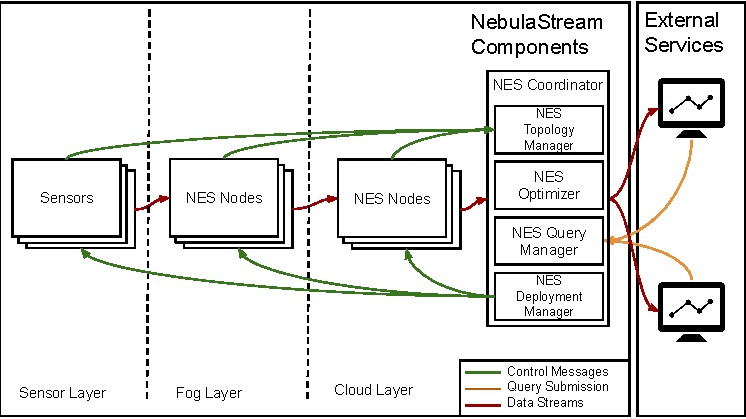
\includegraphics[width=\linewidth]{figs/nes_architecture}
  \caption{Simplified NES architecture overview.}
  \label{nes_architecture}
\end{figure}

Overall, its characteristics allow NES to overcome the limitations of cloud-based SPEs. NES paves the way for a scalable data management back-end for applications in the IoT domain.
